\documentclass{article}
\usepackage[utf8]{inputenc}
\usepackage[a4paper, margin=2cm]{geometry}
\usepackage{multicol, caption}
\usepackage{authblk}
\usepackage[varg]{txfonts}
\usepackage{titlesec}
%\usepackage[T1]{fontenc}
%\usepackage{lmodern}
\usepackage[english]{babel}


\usepackage{amsmath}
\usepackage{amssymb}
\usepackage{amsfonts}
\usepackage{graphicx}% Include figure files
\usepackage{dcolumn}% Align table columns on decimal point
\usepackage{bm}% bold math
\usepackage{hyperref}% add hypertext capabilities
\usepackage{minted}
\usepackage[autostyle]{csquotes}

\usepackage[backend=biber,style=numeric]{biblatex}
\addbibresource{bib.bib}

\hyphenpenalty=10000
\exhyphenpenalty=10000

% CUSTOM FORMAT FOR SECTION
\titleformat{\section}[wrap]{\normalfont\bfseries}{\thesection.}{0.5em}{}
\titlespacing{\section}{12pc}{1.5ex plus .1ex minus .2ex}{1pc}
% CUSTOM SUBSECTION
\titleformat{\subsection}[wrap]{\normalfont\bfseries}{\thesubsection.}{0.5em}{}
\titlespacing{\subsection}{12pc}{1.5ex plus .1ex minus .2ex}{1pc}
% CUSTOM SUBSUBSECTION 
\titleformat{\subsubsection}[wrap]{\normalfont\bfseries}{\thesubsubsection.}{0.5em}{}
\titlespacing{\subsubsection}{12pc}{1.5ex plus .1ex minus .2ex}{1pc}

\newenvironment{Figure}
  {\par\medskip\noindent\minipage{\linewidth}}
  {\endminipage\par\medskip}

\title{PHYS6006 Progress Report \\
       Magnetospheric structure assoiated with high-latitude auroras}
\author[1]{J. Plank}
\author[2]{R. C. Fear}
\affil[1, 2]{Department of Physics and Astronomy, University of Southampton}
\date{January 07, 2020}

\begin{document}
% TITLE BLOCK
\maketitle

% ABSTRACT
\begin{abstract}
    \noindent\textit{Context:} Only case studies have been done on the formation of high latitude aurora, and the connection of interplanetary magnetic field direction is suspected but has never been quantified.\\
    \textit{Aims:} To produce a statistical survey on the relationship between a northward pointing interplanetary magnetic field and a phenomenon known as transpolar arcs.\\
    \textit{Methods:} Using data from Cluster, we analysed the ion temperature for many different values of $Z_{GSM}$, covering the plasma sheet as well as the magnetotail lobes.\\
    \textit{Results:} We found a direct link to IMF direction based on high temperature events observed in the lobe, suggesting high-latitude aruora form during periods of northward pointing IMF.
\end{abstract}

% SWITCH TO 2 COLUMNS
\begin{multicols}{2}

\section{INTRODUCTION}
Earth and the Sun are connected by more than just gravity, magnetic interactions between the two bodies is the cause of some dramatic and complex phenomena. The most well known of these is the aurora (Borealis in the northern hemisphere and Australis in the southern). More commonly known as the northern and southern lights, these fantastical light shows come as a result of charged particles flowing along the magnetic field lines of the Sun and making their way down to Earth in a zone known as an auroral oval \cite{spaceweather}. The violent nature of the Sun can also be transmitted to Earth along its magnetic field, known as the `Interplanetary magnetic field` (IMF). This can result in ``Satellite damage, Radiation hazards to astronauts and airline passengers, telecommunications problems, and outages of power and electronics systems``\cite{spaceweather}. 

The modern theory of the formation of the aurora, into an auroral oval, was first proposed by Hannes Alfvén in 1950. He said that auroras are produced when solar wind encounters the geomagnetic field. The result of this is the formation of the plasmasphere in the equatorial plane of Earth's magnetic field \cite{cosmicelectrodyn}.

\subsection{STRUCTURE OF EARTH'S MAGNETIC FIELD}
Figure \ref{fig:plasmasphere} is a representation of the solar-terrestrial environment. The solar wind, travelling with the interplanetary magnetic field from the sun \cite{Svalgaard_2010}, is coming from the left. It collides with the terrestrial magnetic field at supersonic speeds, creating a bow shock wave in front of the magnetosphere - the region where magnetic field lines connect to Earth at both ends - the boundary of the magnetosphere is the magnetopause. Supersonic solar winds compress at this boundary creating a magnetosheath between the magnetopause and the bow shock \cite{BSPP}.

\begin{Figure}
    \centering
    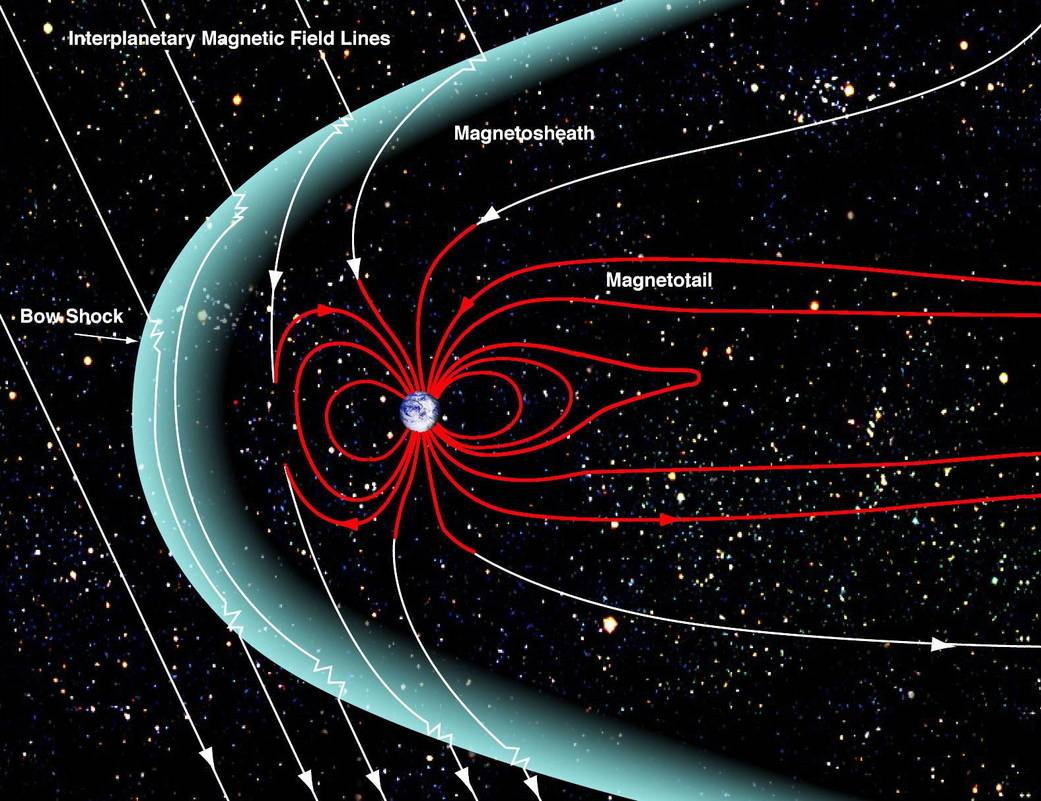
\includegraphics[width=0.8\linewidth]{NASA-Magnetosphere.jpeg}
    \captionof{figure}{Representation of the solar-terrestrial magnetic interaction. The sun is located to the left, producing solar winds and the IMF. Solar winds collide with the terrestrial magnetic field at supersonic speeds, creating a bow shock wave which encases the magnetosphere in a magnetosheath of compressed solar wind \cite{BSPP}. (Image courtesy of NASA)}
    \label{fig:plasmasphere}
\end{Figure}

\subsection{THE INTERPLANETARY MAGNETIC FIELD}
Magnetic field lines are said to be ``frozen in`` to the solar wind plasma, this means the IMF is carried into the interplanetary region of space by solar wind from the sun. The mechanism for this is known as Alfvén's theorem, first proposed in 1942 \cite{alfven_1942}. 

Because of the rotation of the sun, solar wind (along with IMF) follows a spiral pattern similar to that produced by droplets of water as a wet tennis ball is thrown into the air with rapid spin. These field lines are `open`, i.e. they have an origin, but instead of returning to a corresponding region at the opposite pole, extend indefinitely into space \cite{imfUptoLat16}. 

At the magnetic equator, field lines originating from the north and south hemispheres run parallel to each other but are oppositely directed - creating a thin current sheet known as the ``Heliospheric current sheet``. This sheet is twisted and warped due to the difference in rotational and magnetic axes, and a quadrupole moment in the sun's magnetic field - it also has a spiral shape of the same form as described above \cite{alfven_1942, ParkerSpiral}.

Since the orbital plane of the Earth is located almost along the rotation axis of the sun, we experience regular shifts in the direction of flow if the IMF because the heliospheric current sheet is sometimes above and sometimes below the planet. 

When the IMF has a southward component, the northward pointing terrestrial field lines are allowed to merge in a process known as reconnection. However, when the IMF is northward, the structure of the magnetosphere is not well understood \cite{Fear1506}.

\subsection{RECONNECTION AND AURORA}
The auroral lights, pictured in Fig.\ref{fig:auroraPic}, are a result of charged particles from the sun being accelerated towards the ionosphere - Earth's upper atmosphere - where they collide with gas molecules, each molecule causing a different colour to be emitted. 
%E.g. Green (the most common colour) is caused by collisions with atomic oxygen ($557.7 nm$) \cite{hollier, BSPP}. Intense aurora will have an emission rate of several million Rayleigh ($1R=10^6 photons/cm^2s$) and most often appears as east-west aligned bands known as auroral arcs \cite{BSPP}.

\begin{Figure}
    \centering
    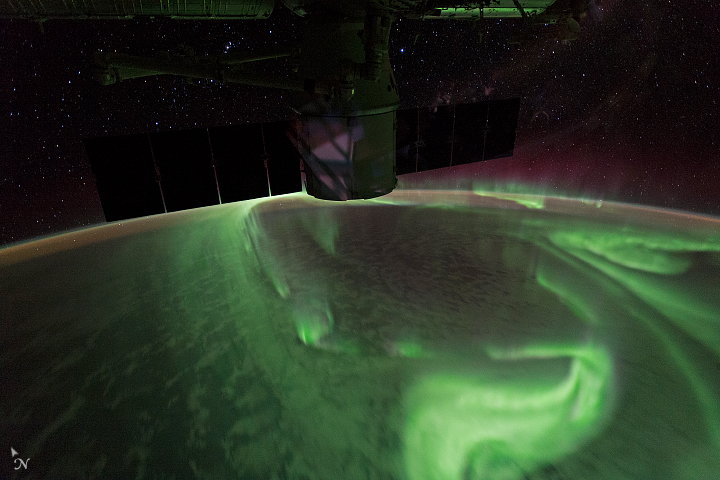
\includegraphics[width=0.8\linewidth]{Aurora_australis_ISS.jpg}
    \captionof{figure}{The Aurora Australis, photographed from the ISS on 19/08/2017. Image from Wikimedia Commons}
    \label{fig:auroraPic}
\end{Figure}

The mechanism allowing ions from the sun to leave the IMF field line they are frozen to and travel down terrestrial ones that enter the ionosphere is reconnection \cite{Angelopoulos931}. Reconnection is a process that allows magnetic fields from separate domains to become joined to one another. When IMF is southward, reconnection occurs in a smooth cycle known as the Dungey cycle \cite{dungeyCycle} which is explained in Fig.\ref{fig:dungey}. Aurora is observed at latitudes of approximately $70^{\circ}$ because that is the boundary between the closed lines and the open ones at the polar cap (lobe).

It is rare to see aurora at very high latitudes, but it can occur in an event known as a transpolar arc \cite{polarAurora1, polarAurora2}. There is much debate on their formation, but the most relevant for this discussion was proposed by Milan et al in \cite{TPAdebate}, where magnetic flux in the magnetotail lobes - the open field line region that maps down to the polar cap - reconnects but is trapped in the magnetotail. Transpolar arcs occur when the IMF is northward, which would explain why flux gets trapped in the magnetotail, there is a blockage created because dayside reconnection cannot occur.

\begin{Figure}
    \centering
    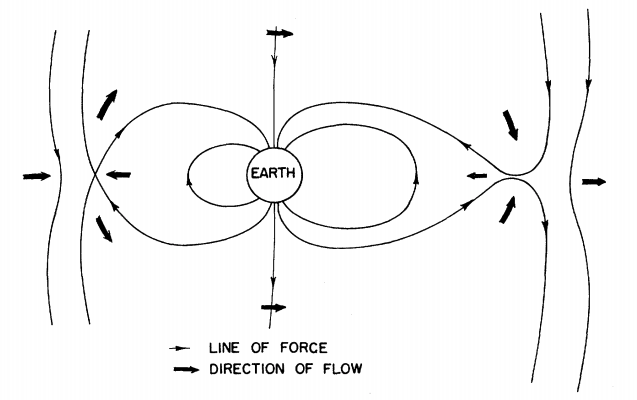
\includegraphics[width=0.8\linewidth]{dungeyCycle.png}
    \captionof{figure}{Sketch of the Dungey cycle. The IMF is assumed to be coming from the left. On the right hand side of the diagram, magnetotail reconnection is happening. Open field lines are being compressed together, eventually joining to form a closed field line that `snaps back` towards Earth, the reconnection happens typically at a radius of $\approx100R_\oplus$. Heating and acceleration of the plasma occurs as the newly created closed field line rapidly shortens in length. The magnetic flux will then flow around to the dayside of the planet (LHS of the sketch) where it gets pushed up against the solar wind. Once again, this pressure eventually reaches a point where the field lines of the IMF and the terrestrial field merge, creating an open line with its foot on the polar cap. This line gets pushed back over to the night-side of the planet where magnetotail reconnection can happen once again. (Sketch from \cite{dungeyCycle})}
    \label{fig:dungey}
\end{Figure}

\subsection{AIMS OF THIS PROJECT}
So far, only case studies have been done on high latitude aurora. The aim of this project is to do a broader statistical survey, the goal being to determine the link between transpolar arc source plasma and the z-direction of the interplanetary magnetic field. To do this, observations were used from ESA's Cluster mission \cite{esaCluster}. Cluster has been providing data on the magnetosphere at high latitudes since February 2001, making it an ideal source for this survey.


\section{OBSERVATIONS}
Since Cluster is designed to achieve many different science goals at once, it necessarily obtains far more data than is necessary for this project. Therefore, the first hurdle was to ascertain the fastest and most reliable way to identify transpolar arc events.

The parameters for the survey were built around the event spotted and analysed in depth by Fear et al in \cite{Fear1506}. This event occurred on the 15th September 2005 between the hours of 1700 and 1900.

\subsection{DETERMINING EVENT SIGNATURES}
Figure \ref{fig:temp_DPF} shows the observed differential particle flux (DPF) and temperature for the month of September 2005. From this we can see the general shape of the data we are working with, including a well recorded event event, occurring in the interval between dashed lines on the ion temperature plot. 

\end{multicols}
\begin{Figure}
    \centering
    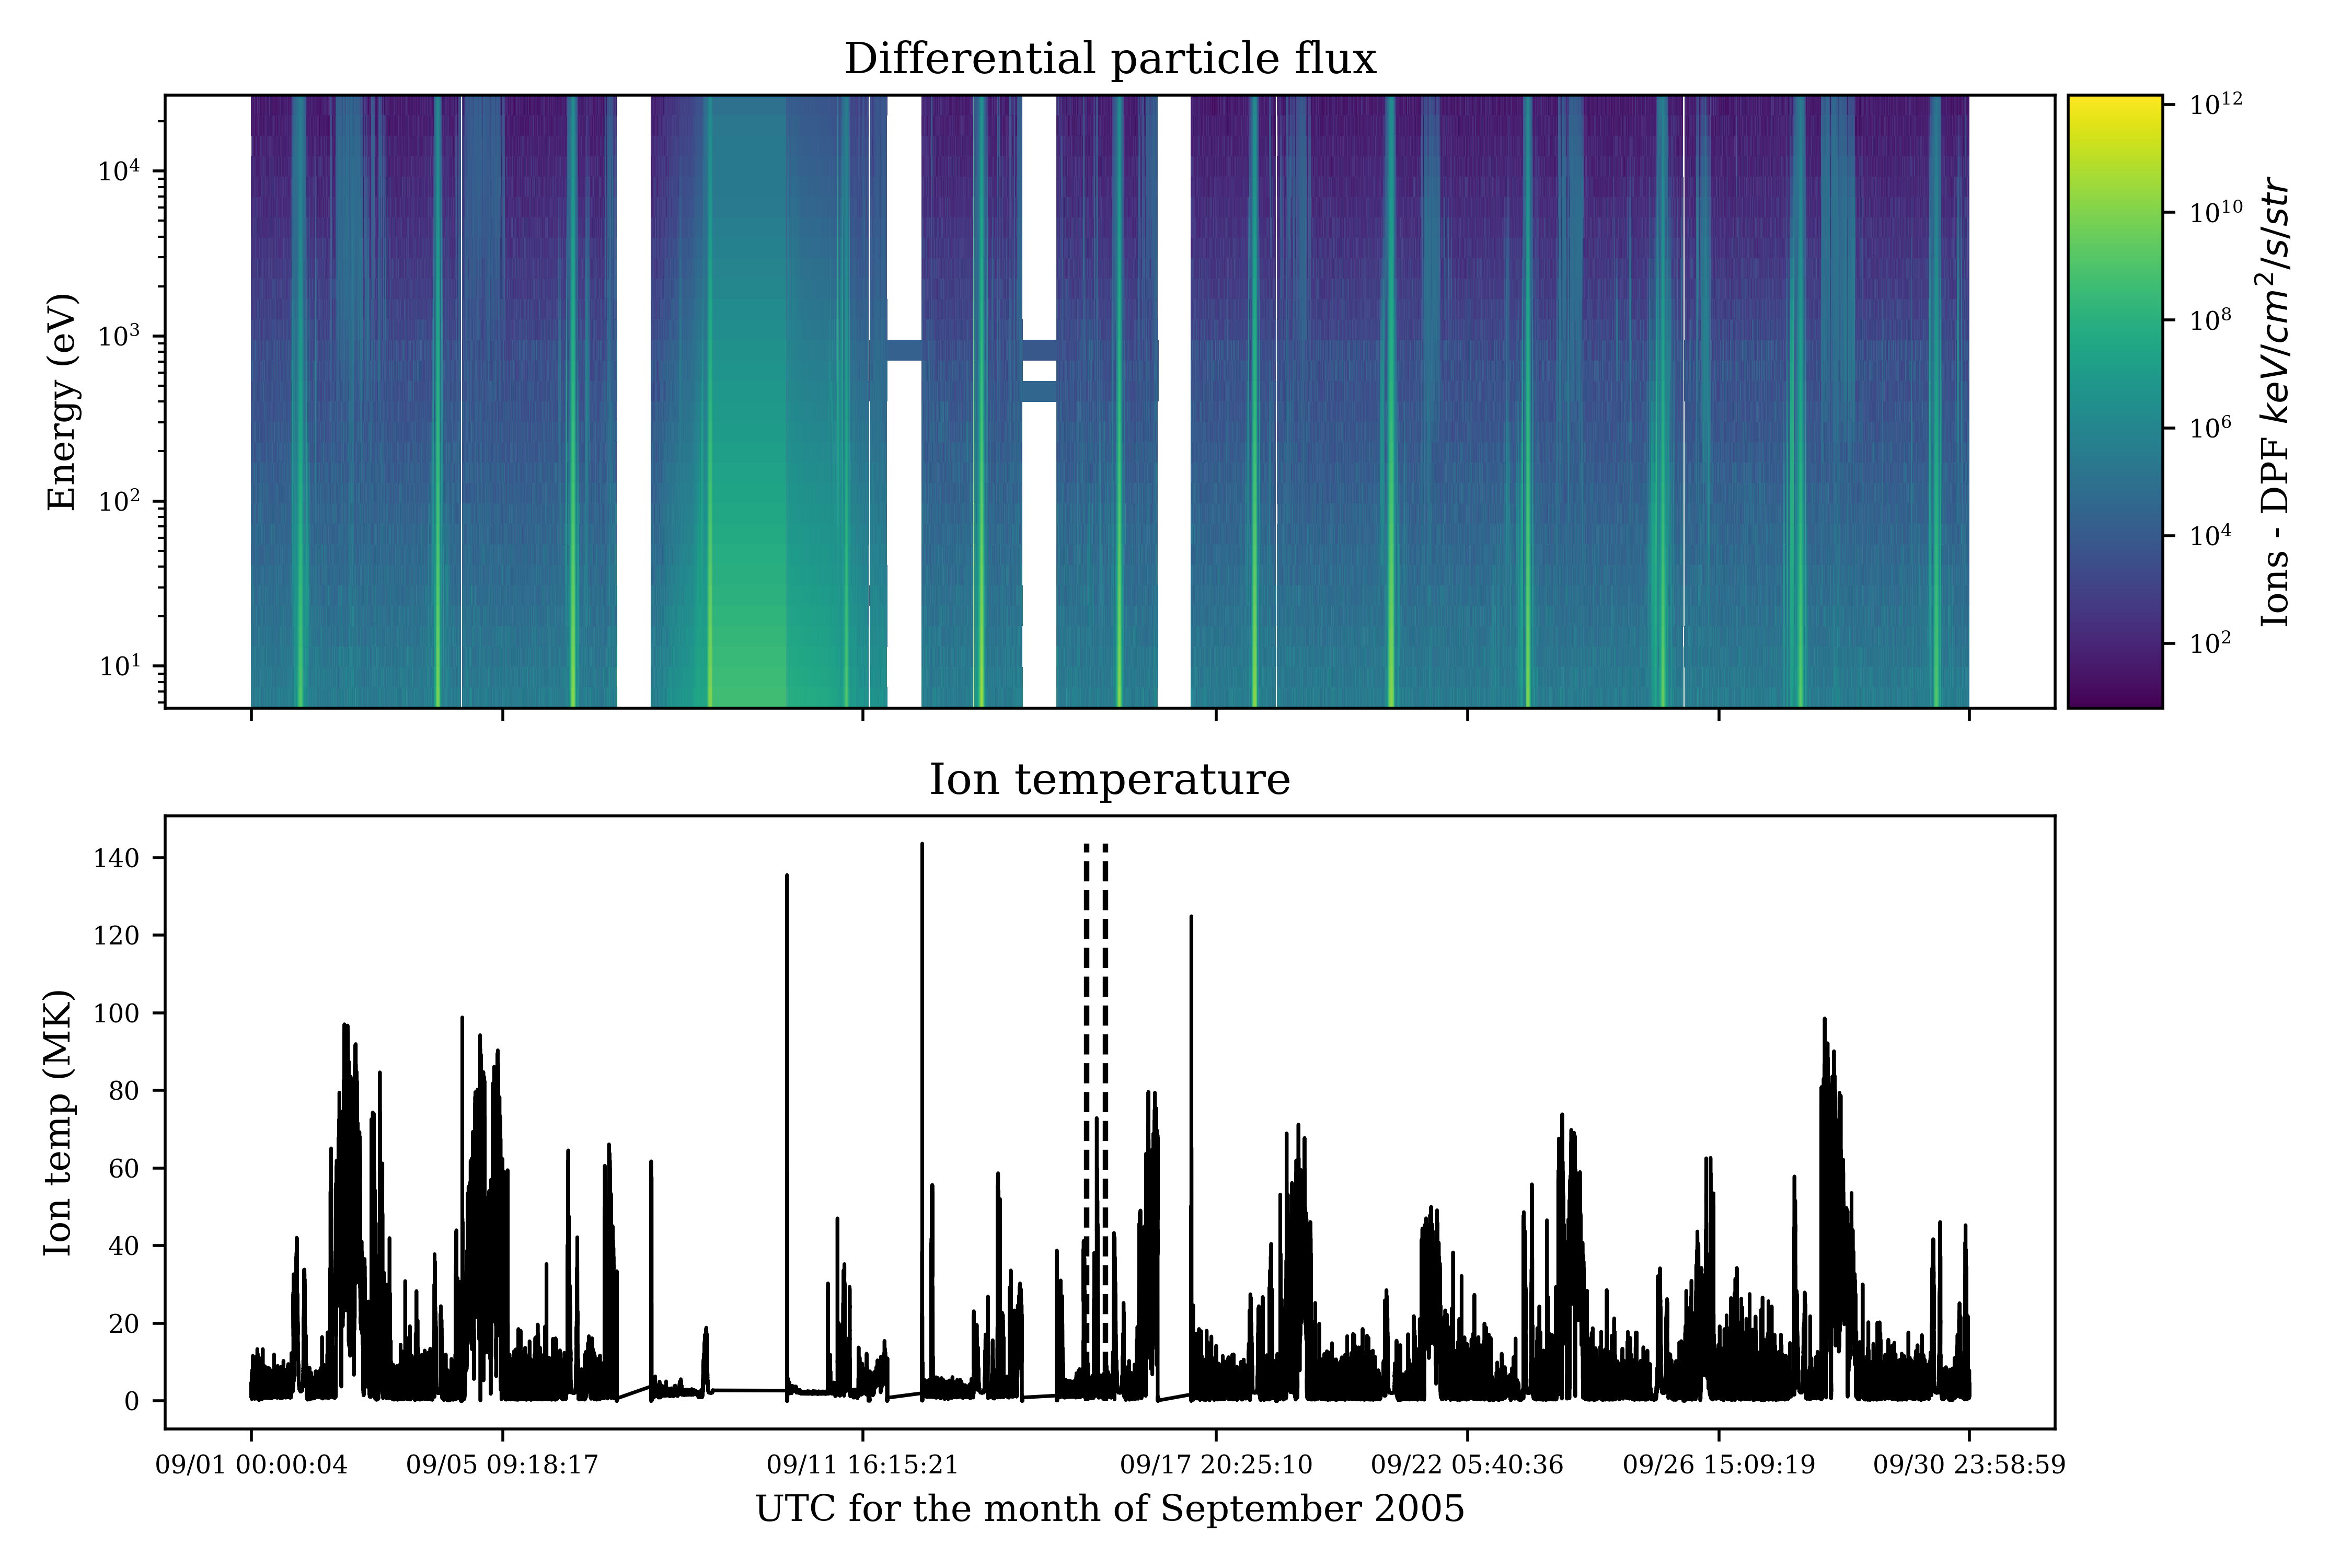
\includegraphics[width=0.8\textwidth]{temp_DPF.png}
    \captionof{figure}{\textbf{Top: Differential particle flux} The x-axis is time, and the y-axis is energy, split into 31 bands. Colour represents differential particle flux (DPF) which, in the scope of this project, can be interpreted as the number of ions at a certain energy. During the event on 15/09/2005 (marked by dashed lines on the bottom plot), we see an increase in high energy ions. This could be used as a signature for a transpolar arc. \textbf{Bottom: Ion temperature} The y-axis here is ion temperature in MK. We see the same periodic increase in temperature associated with the plasma sheet. There are also some brief spikes that are not part of this cycle. Some occur immediately after a period of data loss (most easily seen as areas of white on the DPF plot above) and can be discounted. The 15/09 event was characterised by a temperature spike while Cluster was in the lobe, this is the signature we are looking for
    }
    \label{fig:temp_DPF}
\end{Figure}
\begin{multicols}{2}

Regular spikes in the temperature and DPF (which can be interpreted as the number of ions) can be seen. This is when the spacecraft passes through the plasma sheet (the region of closed field lines from Earth, it is the most active region of the magnetosphere), the source plasma for the traditional auroral oval.

The brief spike occurring on 15/09 is exactly the kind of signature we are looking for \cite{Fear1506}. Since the event shows up just as clearly in the temperature data as in the DPF data, only the temperature readings from cluster will be considered from now on. was based on computational efficiency, since the DPF dataset is massive, loading the observations just from one month took an average of $\approx 98s$. The aim is to expand this analysis to look at many months, for the sake of efficiency we will only consider temperature, which took only $\approx 9s$.

Therefore, an increase in temperature, when the spacecraft is a significant distance from Earth's orbital plane can be considered an indicator for a transpolar arc event. For the remainder of this report, we will consider 

\begin{equation}
    T >= 20MK
\end{equation}

\noindent as the threshold.

\subsection{SPACECRAFT `ALTITUDE`}
Cluster position data was provided by \cite{cdms}. 

We must now consider how Cluster's position in its orbit affects the results we see. Ideally, we would use a regularly updated boundary based on similar parameters as used to generate Fig.\ref{fig:ClusterPos} \cite{substormConfModel}. However, an analysis based purely on Z `altitude` will hopefully reveal a similar trend and has the benefit of simplicity.
\begin{Figure}
    \centering
    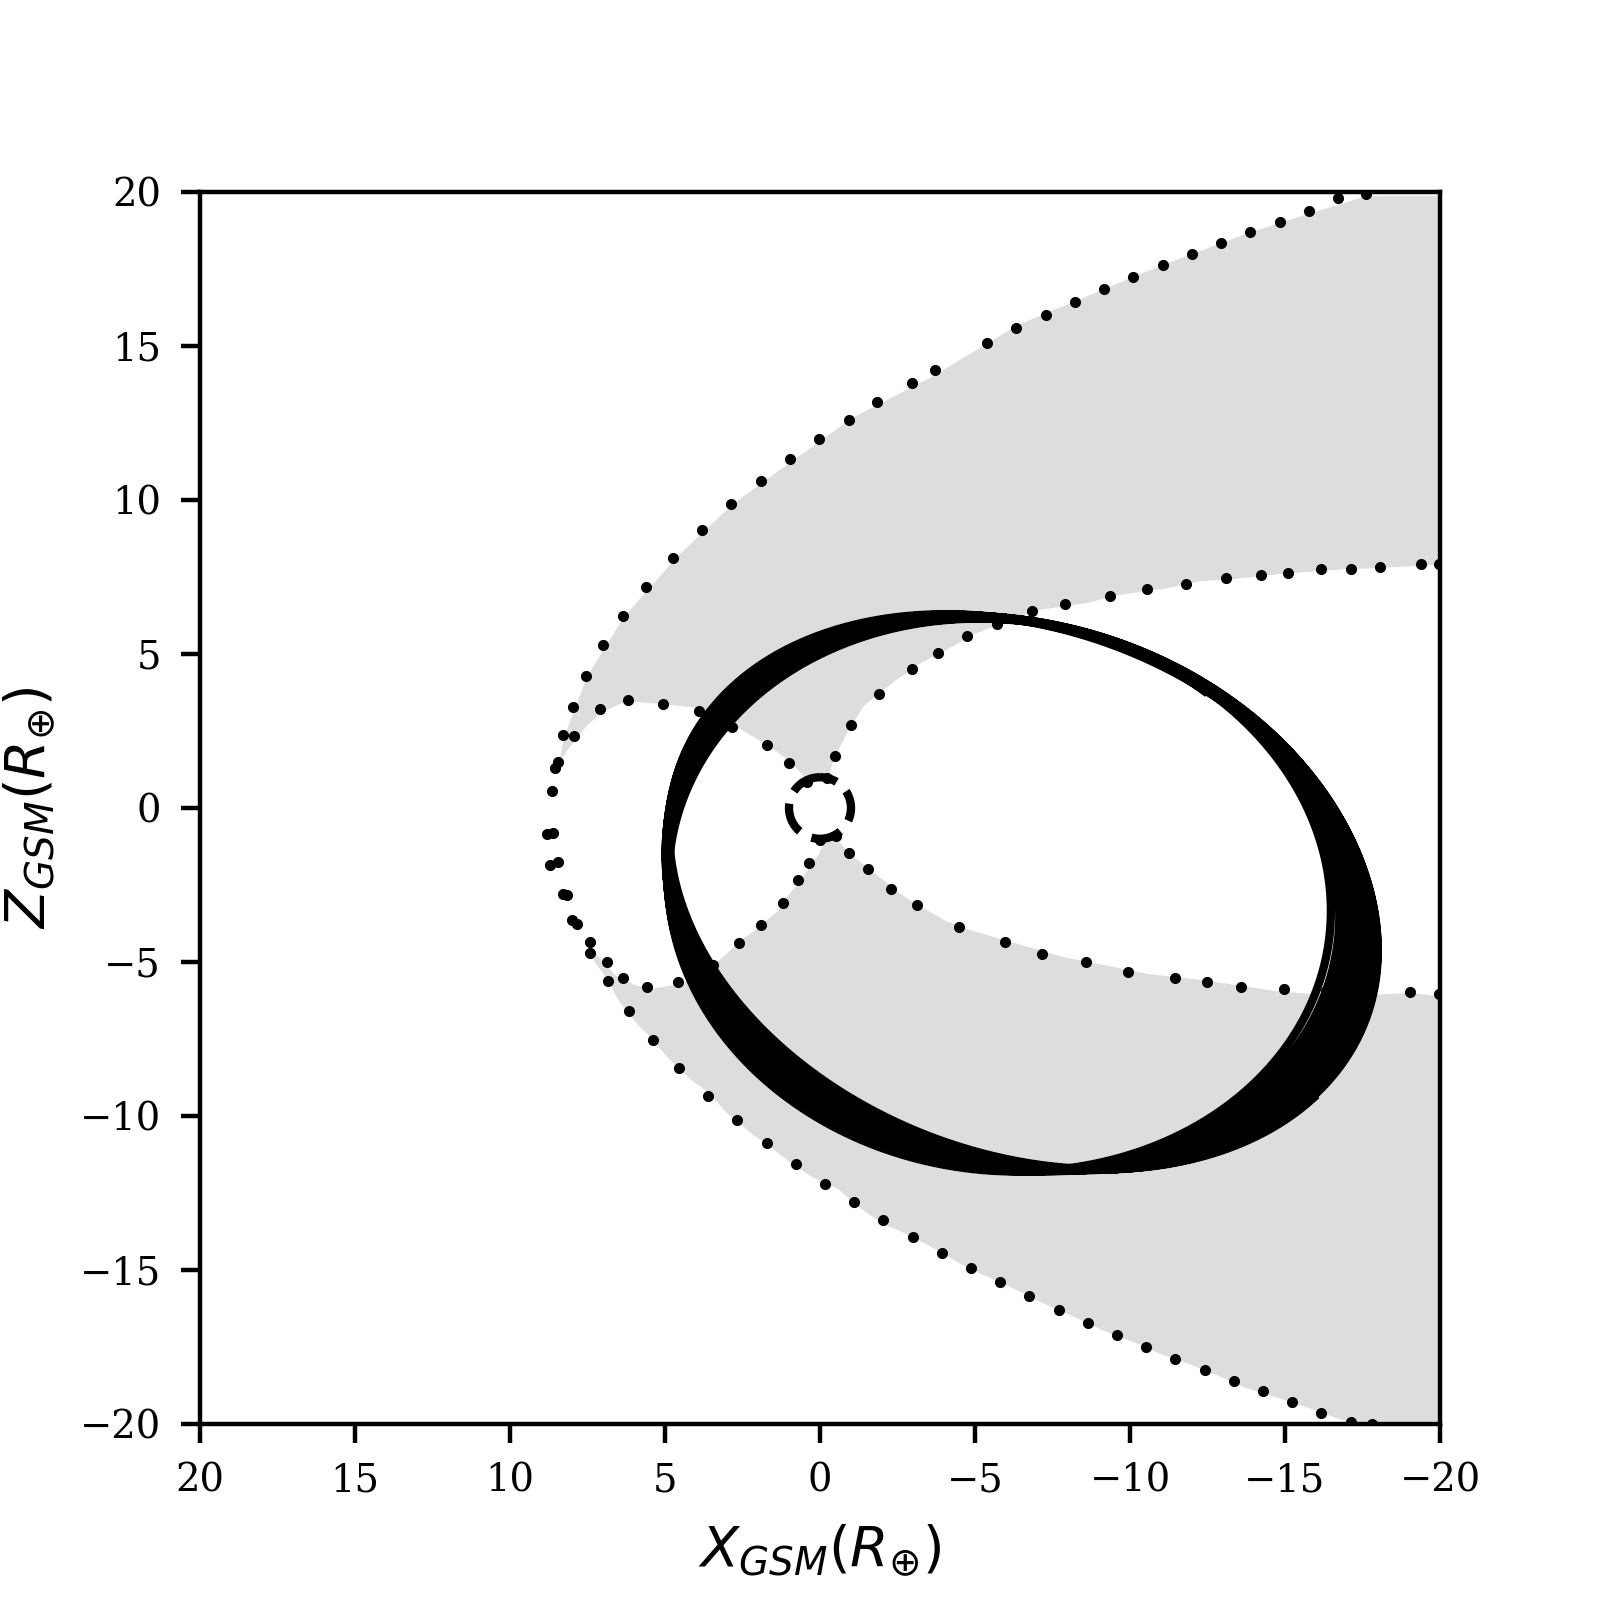
\includegraphics[width=0.75\linewidth]{sc_pos_09_05_coloured.png}
    \captionof{figure}{Plot of Cluster's orbit throughout September 2005 (solid), along with model results for the magnetopause and open-closed boundary on 15/09/2005 (dotted) \cite{Fear1506, substormConfModel}. The grey shaded region is the region of interest as it contains open field lines, if an auroral signature was detected while the spacecraft was in this region then it could indicate a transpolar arc. Plotting is done in the GSM coordinate system, where +X points to the sun and +Z points along the magnetic dipole axis.}
    \label{fig:ClusterPos}
\end{Figure}

\subsection{IMF direction}
IMF data was provided by NASA's OMNI spacecraft. For this report, we are interested in the $B_z$ and $B_y$ components.

\begin{Figure}
    \centering
    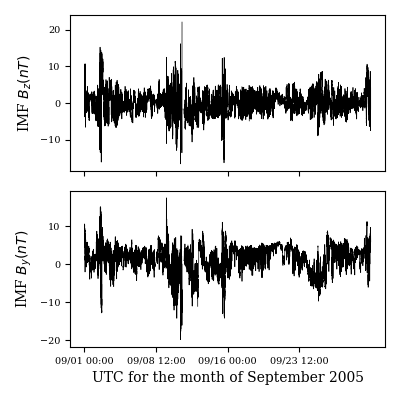
\includegraphics[width=0.6\textwidth]{imf_ts.png}
    \captionof{figure}{Plot of IMF $B_z$ and $B_y$ components for September 2005. The values change very rapidly, the $B_z$ component can change from +ve to -ve on timescales of minutes to hours.}
    \label{fig:IMF_ts}
\end{Figure}

These values can go from positive to negative rapidly, as shown in figure \ref{fig:IMF_ts}. However, the average $B_z$ across an entire month is approximately zero.

\begin{equation}
    \overline{B_z} = 0.13\pm2.95
\end{equation}

\section{RESULTS AND DISCUSSION}
The month of September 2005 was analysed as a starting point since we know that a transpolar arc occurs in this month \cite{Fear1506}.
Fig. \ref{fig:imf_radius} Shows a plot of the variation of average IMF angle as a function of distance from Earth in the GSM z-axis.

Since a numerical mean is not well defined when dealing with angles (as it depends on where the circle is cut), directional statistics was used \cite{mardia_jupp_2000, ClockAngleFear}. First the data was split into overlapping bins such that each one starts at an incrementing multiple of $R_\oplus$, and all end on the maximum $Z_{GSM}$ value. This is so that as you go along the x-axis in figure \ref{fig:imf_radius}, you cut out the lower numbers but still include the higher ones.

At lower altitudes, where the plasma sheet ions are dominant, we see no significant bias towards northward or southward IMF, since the points lie approximately on the $90^\circ$ line. However, at $\approx 5R_\oplus$ there is a sharp change as a northward bias is introduced. This is roughly the boundary line where above this the spacecraft is always in the lobe (Fig.\ref{fig:ClusterPos}).

The average angle was computed by first calculating the clock angle, the angle in the Y-Z plane where $0^\circ$ points at 12 and positive is clockwise. Dawn and dusk conventionally are 9 o'clock and 3 o'clock respectively. Clock angle is given by

\begin{equation}
    \theta_{yz} = \arctan \left(\frac{B_y}{B_z}\right)
\end{equation}

The directional mean of the clock angle is then given by the inverse tangent of the Cartesian coordinates for the centre of mass of the angles (representing unit vectors):

\begin{align}
    \overline{C} &= \frac{1}{n}\sum_{j=1}^n \cos (\theta_j) \\
    \overline{S} &= \frac{1}{n}\sum_{j=1}^n \sin (\theta_j)
\end{align}

\noindent Therefore

\begin{equation}
    \overline{\theta_{yz}} = \arctan \left(\frac{\overline{S}}{\overline{C}}\right)
\end{equation}

\begin{Figure}
    \centering
    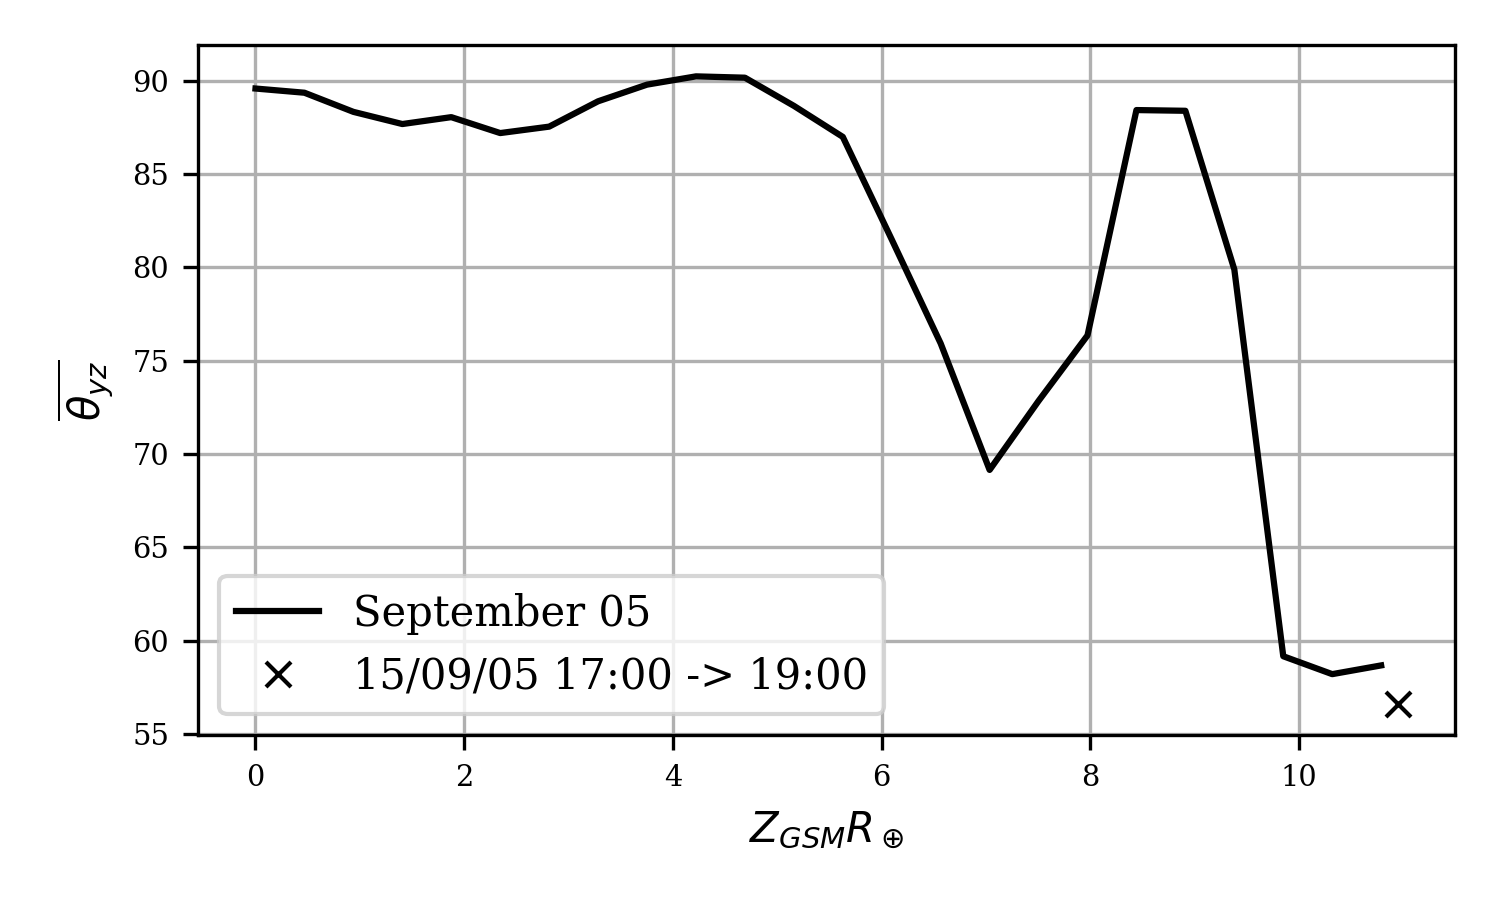
\includegraphics[width=0.8\textwidth]{imf_radius.png}
    \captionof{figure}{Plot of average IMF angle in the Y-Z plane against vertical distance from Earth in $R_\oplus$. The event described in \cite{Fear1506} is marked as a cross. At lower radii we see what is expected i.e. the angle is somewhere close to $90^\circ$, indicating little bias from $B_z$. At around $5R_\oplus$ there is a sharp change in angle as the IMF suddenly becomes northward. This is in support of the hypothesis that auroral signatures in the lobes are linked to northward IMF. Note: Angles were folded into the range $0\rightarrow180$ to avoid any confusing oscillations as the average crosses the $0\rightarrow360^\circ$ boundary. See Fig.\ref{fig:imf_radialHist} for a more complete picture.}
    \label{fig:imf_radius}
\end{Figure}

Figure \ref{fig:imf_radialHist} shows a collection of histograms of the IMF clock angle distribution. These show a much more complete picture of how the average evolves. There appears to be a bias towards positive $B_y$. This can be explained simply by Fig.\ref{fig:imf_cartHist}, the total IMF, $B_y$ component was biased for September 05, regardless of temperature, altitude, etc...

\begin{Figure}
    \centering
    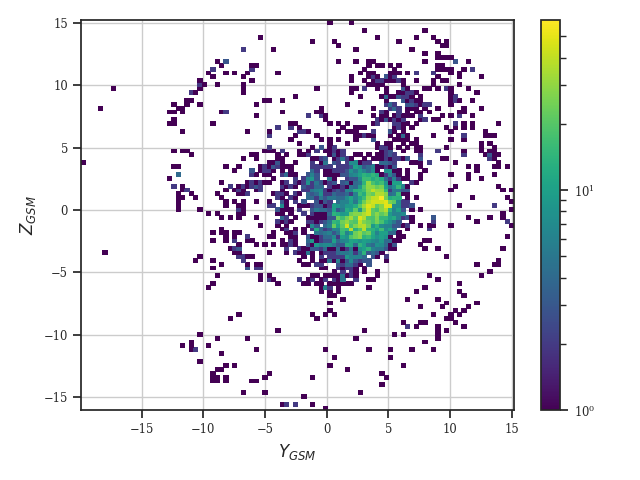
\includegraphics[width=0.8\textwidth]{imf_cartHist.png}
    \captionof{figure}{Plot of the IMF distribution for September 2005, in terms of $B_y$ and $B_z$. The Z component is centred well on 0 displacement, but the y component is clearly has a positive bias.}
    \label{fig:imf_cartHist}
\end{Figure}

\section{CONCLUSION: FUTURE WORK}
As was made clear from analysis of figures \ref{fig:imf_radius} and \ref{fig:imf_radialHist}, there is a need for more data. The hope is that with a larger data-set there will be less uncertainty in the result. This is a very logical continuation of the project and will likely be the primary focus going forward.

A useful further extension would then be to couple this with low-altitude plasma observations in order to confirm a statistical link between these events and transpolar arc formation.

\end{multicols}
\begin{figure*}
    \centering
    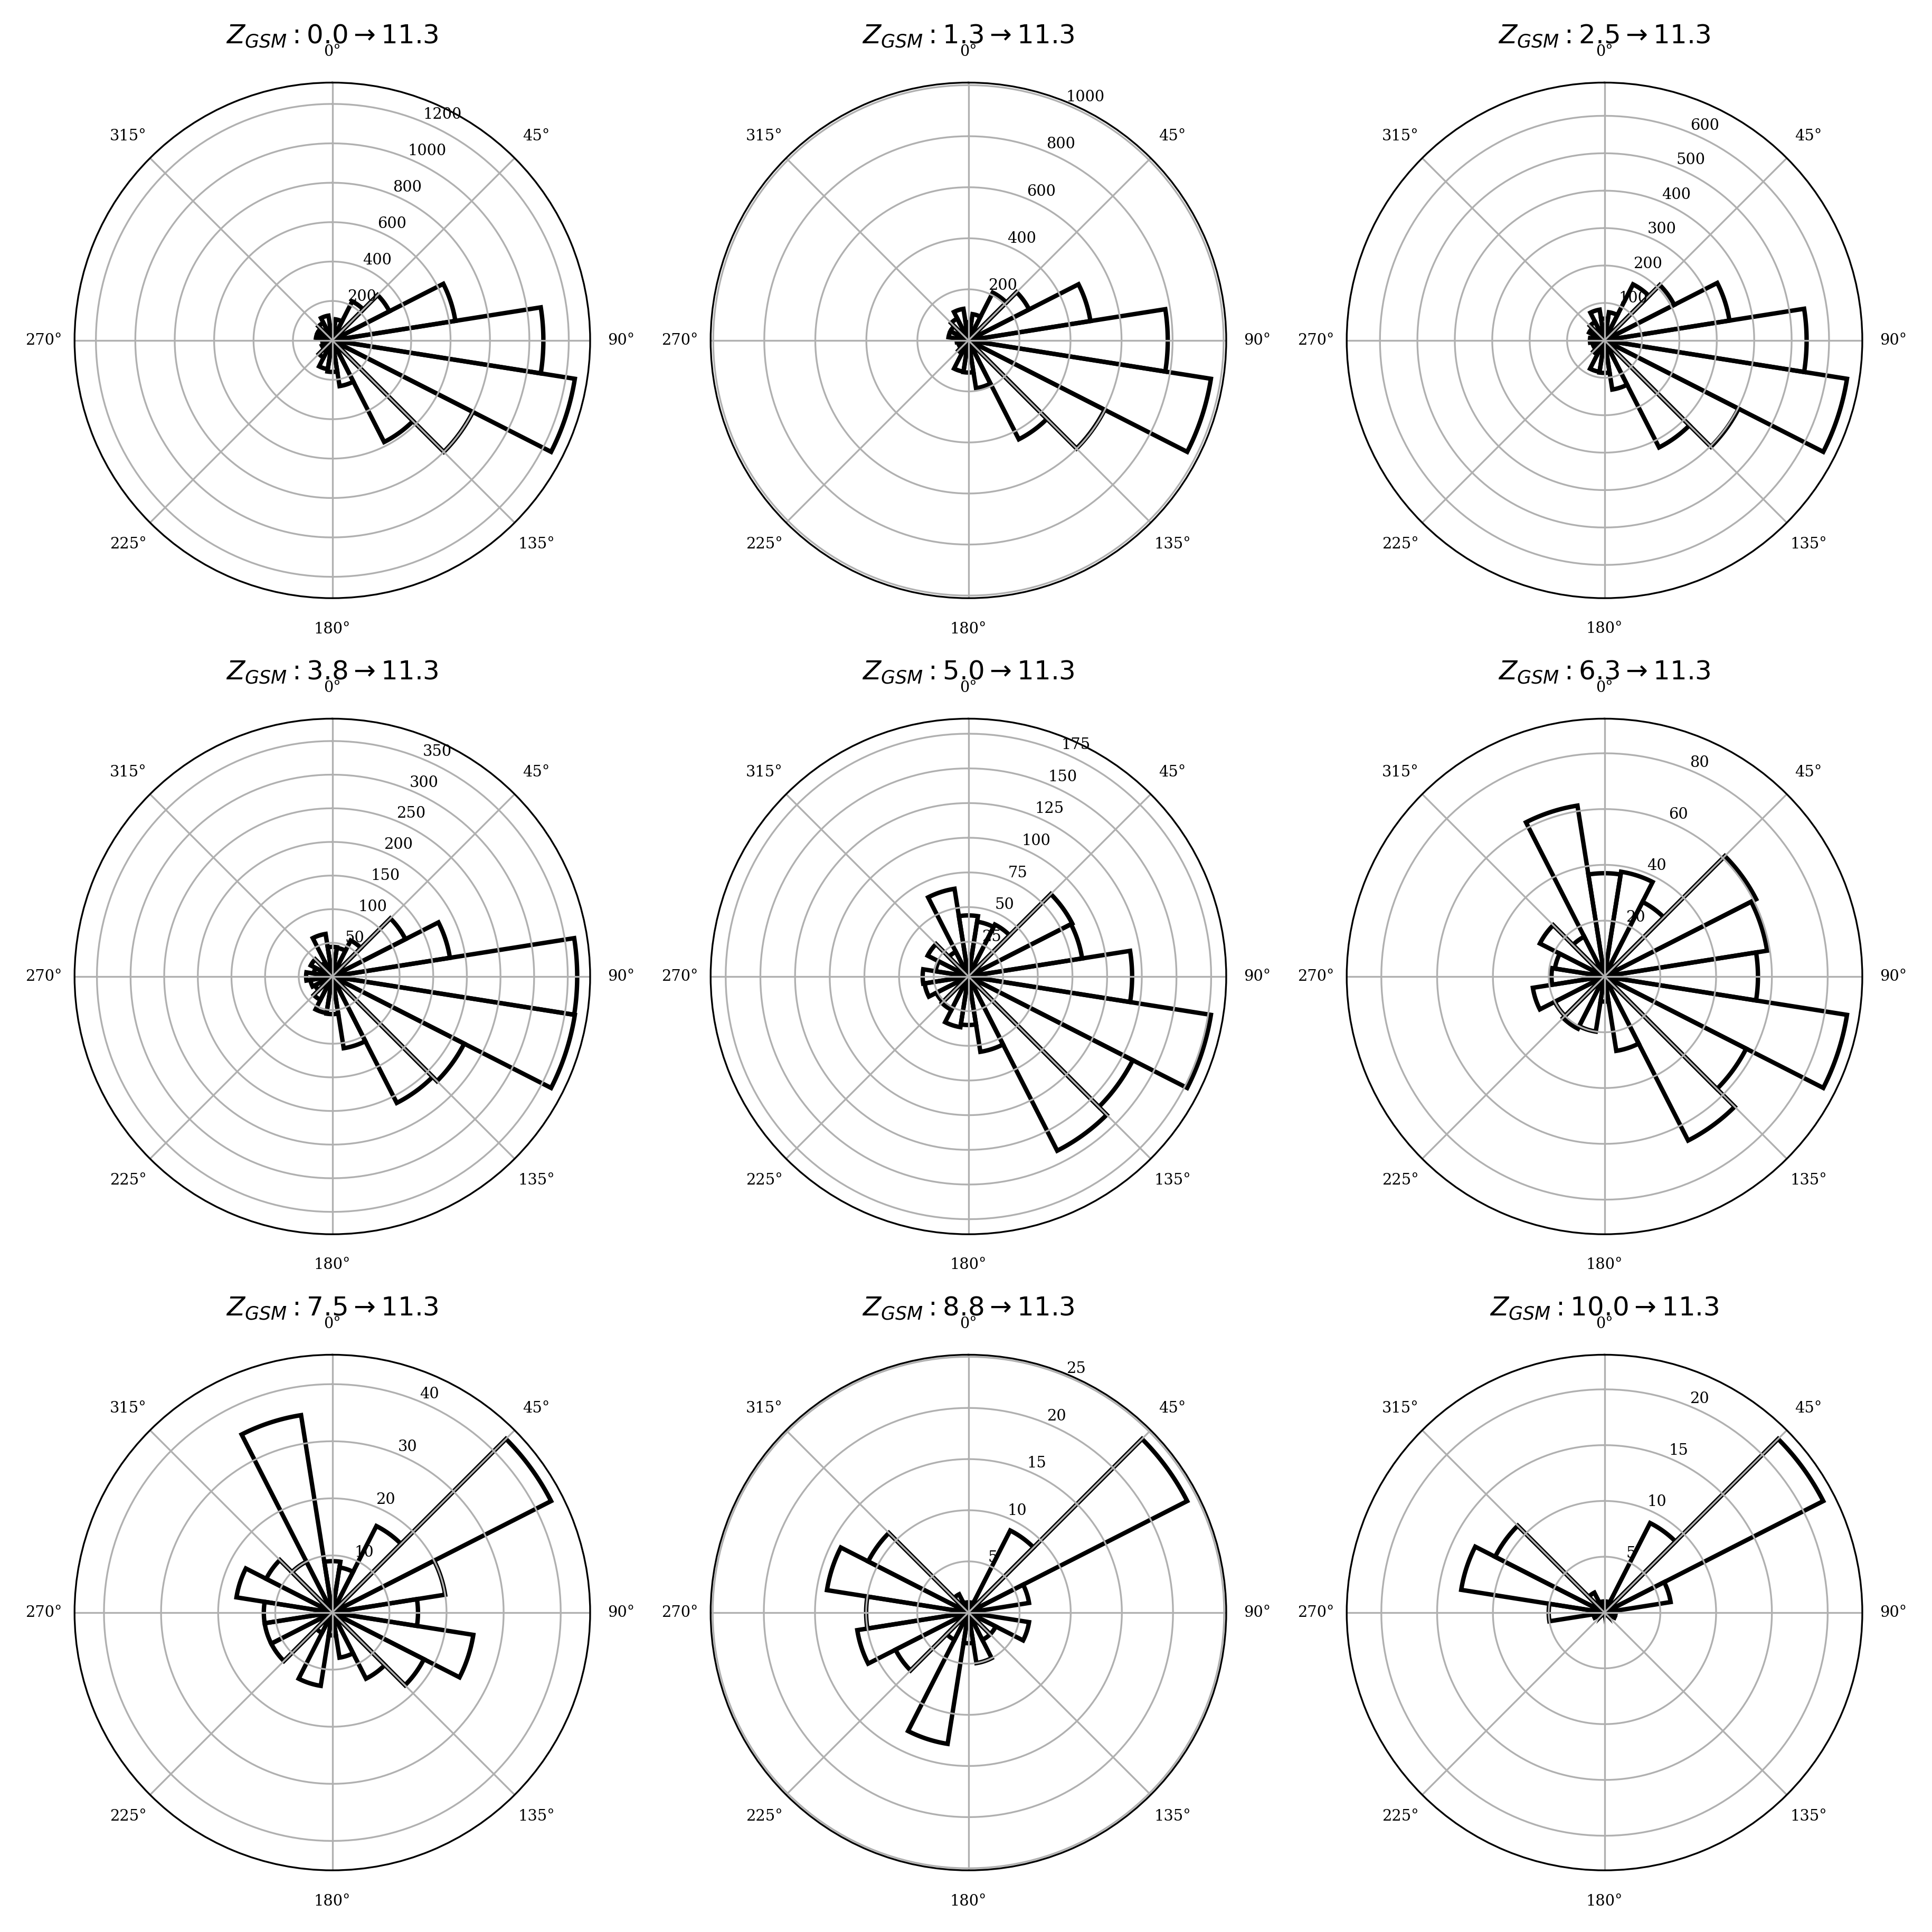
\includegraphics[width=0.9\linewidth]{imf_radialHistGSM.png}
    \caption{Clock angle distributions at various $Z_{GSM}$ showing the evolution as radius is increased. The length of each bar corresponds to the number of samples with that angle. There is a clear bias towards $90^\circ$, introduced because of a general bias in the data for September 2005.}
    \label{fig:imf_radialHist}
\end{figure*}
\begin{multicols}{2}

\printbibliography
\end{multicols}
\end{document}